\setchapterpreamble[u]{\margintoc}
\chapter{Introduction}
\labch{intro}
% Motivation and preparation for structure

% Paragraphs:

% Context for less familiar readers, broad anchor in space & time
In 1896 the Dutch physicist Pieter Zeemann discovered that the visible spectral lines of a mercury vapour lamp split up in the presence of a magnetic field \sidecite{zeemanInfluenceMagnetismNature1896}. In 1938 Isidor Rabi then first described nuclear magnetic resonance \sidecite{rabiNewMethodMeasuring1938}. His technique was in turn extended by Felix Bloch \sidecite{blochNuclearInductionExperiment1946} and Edward Mills Purcell \sidecite{purcellResonanceAbsorptionNuclear1946} and is nowadays one of the most powerful tools in analytical sciences. It can be used for analysing the structure of molecular systems, studying crystals and imaging in medicine among others. In 1966 Richard Robert Ernst developed Fourier transform nuclear magnetic resonance spectroscopy (FT-NMR) \sidecite{ernstApplicationFourierTransform1966}, which is the same fundamental technique used today.

Since then, technology has advanced fast to higher magnetic field strengths and higher processing power. Enabling better images, higher resolutions and new technology magnetic resonance has become an essential part of many scientists' toolboxes. Unfortunately, higher capabilities come hand in hand with higher costs.

Not much effort has gone towards using the technological advancements of recent decades to lower the cost of magnetic resonance technology. Therefore, there are myriads of lost opportunities in education, industry and research. This can be seen easily when looking at the number of NMR publications published in a given country in \reffig{nmr_citations}.
\begin{figure*}[h!bt]
    \centering
    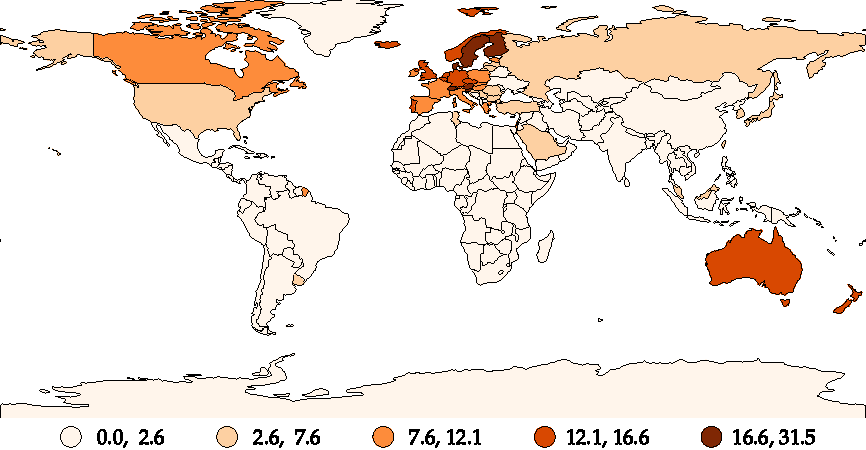
\includegraphics{data/nmr_citations/nmr-affiliations-per-million-people_naturalbreaks.pdf}
    \caption{\captiontitle{\enquote{NMR publications} per million capita (2021)}. White countries have no access to NMR, while Switzerland appears as a global leader in NMR science. (Dr. Maria Pechlaner, Infozentrum Chem. Biol. Pharm., ETH Zürich; database: Scopus)}
    \labfig{nmr_citations}
\end{figure*}
This is in line with the growing disparity in citations \sidecite{nielsenGlobalCitationInequality2021}.

% Need for the work, i.e. what the scientific community has vs what they want
Consequently, this work focuses on lowering the entry barrier to magnetic resonance research, specifically nuclear magnetic resonance spectroscopy (NMR).

% Indicate what I have done (i.e. the task)

% Preview of the paper to prepare for structure



\section{Concept}
Idea/motivation
given magnet
schema of setup
Design decisions
rf switch
amplifiers

\section{Complete Setup}

\begin{circuitikz}[european]
    \ctikzset{bipoles/amp/width=0.9}
    \draw[nodes={align=center}]
    (0,0) coordinate(mid)

    % TX
    (mid) ++(0,3) node[draw, align=center, minimum height=5.5cm, minimum width=2cm](decoder){Sequence\\Decoder}
    ($(decoder.east)!0.75!(decoder.north east)$) coordinate(decoderi)
    ($(decoder.east)!0.75!(decoder.south east)$) coordinate(decoderq)
    ($(decoder.north west)!0.5!(decoder.south west)$) coordinate(decoderin)
    (decoderin) ++(-1,0) node[left]{Pulse\\Sequence} coordinate(seq) -- (decoderin) node[inputarrow]{}
    (decoderi) node[left]{I} ++(3,0) node[mixer](mi1){}
    (decoderq) node[left]{Q} ++(3,0) node[mixer](mq1){}
    (decoderi) -- (mi1.w) node[inputarrow]{}
    (decoderq) -- (mq1.w) node[inputarrow]{}
    (decoderin -| mi1.s) coordinate (center1)
    (center1) ++(-1,0) node[oscillator](osc1){} -- (center1) -- (mi1.s) node[inputarrow,rotate=90]{}
    (osc1.n) node[above]{NCO}
    (osc1.s) node[below]{\qty{25}{MHz}}
    (center1) to[phaseshifter,>,l=90°] (mq1.n) node[inputarrow,rotate=270]{}
    (center1) ++(2,0) node[adder](add1){}
    (mi1.e) -| (add1.n) node[inputarrow,rotate=270]{}
    (mq1.e) -| (add1.s) node[inputarrow,rotate=90]{}
    (add1.e) to[dac,>] ++(2,0) to[amp,t=PA,l=Power\\Amplifier,>] ++(2,0) coordinate(tx)

    % Circulator
    (mid -| tx) node[circulator](circ){} node[below right]{passive\\TX/RX Switch}
    (tx) -| (circ.n) node[inputarrow,rotate=270]{}

    % RX
    (mid) ++(0,-3) coordinate(center_rx)
    (center_rx -| circ) coordinate(rx_out)
    (circ.s) |- (rx_out)
    (rx_out) to[amp,t=\rotatebox{180}{LNA},l=Low Noise\\Amplifier,>] ++(-2,0) to[adc,>] ++(-2,0) -- (rx_out -| add1) coordinate(rx_split)
    (rx_split) ++(0,2) coordinate(rx_upper)
    (rx_split) ++(0,-2) coordinate(rx_lower)
    (rx_upper -| mi1) node[mixer](mi2){}
    (rx_lower -| mq1) node[mixer](mq2){}
    (rx_split) |- (mi2.e) node[inputarrow,rotate=180]{}
    (rx_split) |- (mq2.e) node[inputarrow,rotate=180]{}
    (rx_split -| osc1) node[oscillator](osc2){}
    (osc2.n) node[above]{NCO}
    (osc2.s) node[below]{\qty{25}{MHz}}
    (osc2.e) -| (mi2.s) node[inputarrow,rotate=90]{}
    (osc2.e -| mq2) to[phaseshifter,>,l=90°] (mq2.n) node[inputarrow,rotate=270]{}
    (mi2.w) to[bandpass,l_=CIC,>] (mi2 -| decoderi) node[inputarrow,rotate=180]{} node[left](circ_out_i){I}
    (circ_out_i) -- (mi2 -| seq) node[left]{I} node[inputarrow,rotate=180]{}
    (mq2.w) to[bandpass,l=CIC,>] (mq2 -| decoderq) node[inputarrow,rotate=180]{} node[left](circ_out_q){Q}
    (circ_out_q) -- (mq2 -| seq) node[left]{Q} node[inputarrow,rotate=180]{}

    % Probe
    (circ.e) -- ++(2,0) node[dinantenna](probe){Probe}
    ;

    % Red Pitaya
    \draw[dashed]
    ($(seq)!0.5!(decoderin)$) ++(0,3) coordinate(rectangle_start)
    ($(add1.e)!0.5!(tx)$) coordinate(rp_out)
    (rp_out |- mq2) ++(0,-1) coordinate(rectangle_end)
    (rectangle_start) rectangle (rectangle_end)
    (rectangle_start) node[above right]{Red Pitaya}
    ;
\end{circuitikz}